\documentclass[12pt,a4paper]{report}
\usepackage[T2A]{fontenc}
\usepackage[utf8]{inputenc}
\usepackage[russian]{babel}
\usepackage{graphicx, setspace, amsmath}
\usepackage{minted}

\usepackage[
top = 1.25cm,
bottom = 2.0cm]{geometry}

\begin{document}
\begin{titlepage}
    \centering
    % HEADER
    {
        \scshape
        Федеральное государственное автономное образовательное учреждение высшего образования
        \par
        \textbf{«Научно-образовательная корпорация ИТМО»}
        \par
        \vspace*{1cm}
        Факультет Программной Инженерии и Компьютерной Техники
        \par
    }
    % LOGO
    \vspace*{0.6cm}
    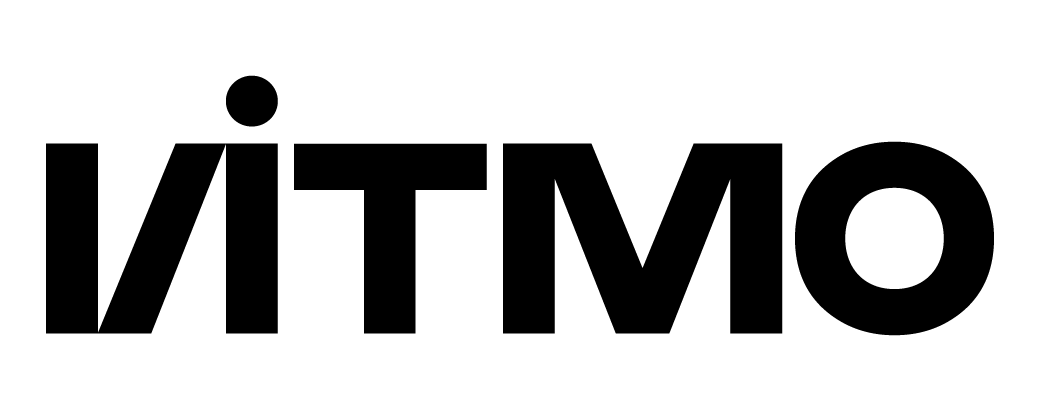
\includegraphics[width=\textwidth]{logo.png}
    % LAB INFO
    {
        \Large
        \textbf{Лабораторная работа по\\<<Тестированию программного обеспечения>> №2}
        \par
        \normalsize
        \vspace*{0.75cm}
        \textbf{Вариант 18450}
        \par
    }
    \vfill
    % СREDITS
    \hfill\begin{minipage}{\dimexpr\textwidth-7.8cm}
        \textbf{Выполнил:}\par
        Степанов Арсений Алексеевич\par
        \vspace*{0.15cm}
        \textbf{Группа:}\par
        P3318\par
        \vspace*{0.15cm}
        \textbf{Преподаватель:}\par
        Егошин Алексей Васильевич\par
    \end{minipage}
    \vfill
    Санкт-Петербург, \the\year{}г.
\end{titlepage}

\section*{Задание}
Провести интеграционное тестирование программы, осуществляющей вычисление системы функций:
$$
    \begin{cases}
        x \leq 0 : \tan x \\
        x > 0 : \dfrac{\left(\dfrac{\log_5 x}{\ln x} - \log_3 x\right)^2}{\log_5 x} \log_3 x
    \end{cases}
$$
\subsection*{Правила выполнения работы}
\begin{enumerate}
    \item Все составляющие систему функции (как тригонометрические, так и логарифмические) должны быть выражены через базовые (тригонометрическая зависит от варианта; логарифмическая - натуральный логарифм)
    \item Структура приложения, тестируемого в рамках лабораторной работы, должна выглядеть следующим образом:
          \begin{center}
              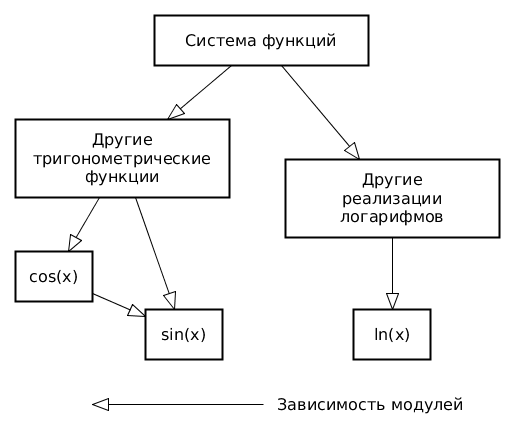
\includegraphics[width=0.75\textwidth]{assets/schema.png}
          \end{center}
    \item Обе базовые функции (в примере выше - $\sin x$ и $\ln x$) должны быть реализованы при помощи разложения в ряд с задаваемой погрешностью. Использовать тригонометрические / логарифмические преобразования для упрощения функций запрещено
    \item Для каждого модуля должны быть реализованы табличные заглушки. При этом, необходимо найти область допустимых значений функций, и, при необходимости, определить взаимозависимые точки в модулях
    \item Разработанное приложение должно позволять выводить значения, выдаваемое любым модулем системы, в сsv файл вида <<X, Результаты модуля (X)>>, позволяющее произвольно менять шаг наращивания Х. Разделитель в файле csv можно использовать произвольный
\end{enumerate}

\newpage
\section*{Выполнение}
\subsection*{Функции текущей реализации}
В текущей реализации и тестах используются следующие функции: \texttt{sin}, \texttt{cos}, \texttt{tan}, \texttt{ln}, \texttt{log\_3}, \texttt{log\_5}, \texttt{complex}.

\subsection*{Обоснование покрытия}
\subsubsection*{Стратегия интеграционного тестирования}
Для тестирования системы функций была выбрана стратегия Top-Bottom, так как реализовать
заглушки для функций целесообразнее и проще, нежели драйвера вышестоящих функций. Достаточно
просто заменить какую-либо из функций на её табличную заглушку. При тестировании реальные вызовы
функций заменяются на заглушки использующие табличные значения

\subsubsection*{Система функций}
\begin{enumerate}
    \item Классы эквивалентности:
          \begin{itemize}
              \item Ветвь $x \le 0$: функция равна \texttt{tan(x)}
              \item Ветвь $0 < x < 1$: правая часть формулы
              \item Ветвь $x > 1$: правая часть формулы
          \end{itemize}
    \item Граничные случаи:
          \begin{itemize}
              \item Точка переключения ветвей $x=0$
              \item Разрыв \texttt{tan} на $x=-\pi/2$ в левой ветви
              \item Точка разрыва правой ветви в $x=1$
              \item \texttt{NaN}, $+\infty$, $-\infty$
              \item Перегрузка для целых типов
          \end{itemize}
\end{enumerate}
\begin{center}
    \begin{tabular}{|c|c|c|}
        \hline
        \textbf{f} & \textbf{Вход} & \textbf{Ожидаемый результат} \\
        \hline
        \texttt{complex} & $-2.0$ & $-7.0$ \\
        \hline
        \texttt{complex} & $-0.5$ & $-1.5$ \\
        \hline
        \texttt{complex} & $0.0$ & $0.25$ \\
        \hline
        \texttt{complex} & $0.5$ & $2.0583673469387755$ \\
        \hline
        \texttt{complex} & $2.0$ & $6.797819492680379 \cdot 10^{-5}$ \\
        \hline
        \texttt{complex} & $5.0$ & $1.0274355640600286$ \\
        \hline
        \texttt{complex} & $-\pi/2$ & \texttt{NaN} \\
        \hline
        \texttt{complex} & $1.0$ & \texttt{NaN} \\
        \hline
        \texttt{complex} & $+\infty$ & \texttt{NaN} \\
        \hline
    \end{tabular}
\end{center}

\subsubsection*{Функция \texttt{cos}}
\begin{enumerate}
    \item Классы эквивалентности:
          \begin{itemize}
              \item Конечные значения из разных областей
              \item Эквивалентность по периодичности $2\pi$
              \item Симметричная пара $x$ и $-x$
          \end{itemize}
    \item Граничные случаи:
          \begin{itemize}
              \item Характерные точки $0$, $\pi/2$, $\pi$, $2\pi$
              \item Специальные входы \texttt{NaN}, $+\infty$, $-\infty$
              \item Перегрузка для целых типов
          \end{itemize}
\end{enumerate}
\begin{center}
    \begin{tabular}{|c|c|c|}
        \hline
        \textbf{f} & \textbf{Вход} & \textbf{Ожидаемый результат} \\
        \hline
        \texttt{cos} & $-1.0$ & $1.234$ \\
        \hline
        \texttt{cos} & $0.0$ & $0.321$ \\
        \hline
        \texttt{cos} & $1.0$ & $-0.654$ \\
        \hline
        \texttt{cos} & $\pi/2$ & $0.0$ \\
        \hline
        \texttt{cos} & $\pi$ & $-0.7$ \\
        \hline
        \texttt{cos} & $2\pi$ & $0.321$ \\
        \hline
        \texttt{cos} & \texttt{NaN} & \texttt{NaN} \\
        \hline
        \texttt{cos} & $+\infty$ & \texttt{NaN} \\
        \hline
    \end{tabular}
\end{center}

\subsubsection*{Функция \texttt{ln}}
\begin{enumerate}
    \item Классы эквивалентности:
          \begin{itemize}
              \item Положительные значения $0 < x < 1$
              \item Точка $x=1$
              \item Положительные значения $x > 1$
          \end{itemize}
    \item Граничные случаи:
          \begin{itemize}
              \item $x=0$ и окрестность $0^+$
              \item Отрицательные $x$
              \item \texttt{NaN} и $+\infty$
              \item Характерные точки $e$ и $e^2$
              \item Перегрузка для целых типов
          \end{itemize}
\end{enumerate}
\begin{center}
    \begin{tabular}{|c|c|c|}
        \hline
        \textbf{f} & \textbf{Вход} & \textbf{Ожидаемый результат} \\
        \hline
        \texttt{ln} & $0.1$ & $-2.3025850929940455$ \\
        \hline
        \texttt{ln} & $0.5$ & $-0.6931471805599453$ \\
        \hline
        \texttt{ln} & $1.0$ & $0.0$ \\
        \hline
        \texttt{ln} & $2.0$ & $0.6931471805599453$ \\
        \hline
        \texttt{ln} & $10.0$ & $2.302585092994046$ \\
        \hline
        \texttt{ln} & $0.0$ & $-\infty$ \\
        \hline
        \texttt{ln} & $-1.0$ & \texttt{NaN} \\
        \hline
        \texttt{ln} & $+\infty$ & $+\infty$ \\
        \hline
    \end{tabular}
\end{center}

\subsubsection*{Функции \texttt{log\_3} и \texttt{log\_5}}
\begin{enumerate}
    \item Классы эквивалентности:
          \begin{itemize}
              \item Положительные $x$ из диапазона $0 < x < 1$.
              \item Точка $x=1$.
              \item Положительные $x > 1$.
          \end{itemize}
    \item Граничные случаи:
          \begin{itemize}
              \item Характерные точки оснований: $3$, $9$ и $5$, $25$
              \item $x=0$, отрицательные $x$
              \item \texttt{NaN} и $+\infty$
              \item Перегрузка для целых типов
          \end{itemize}
\end{enumerate}
\begin{center}
    \begin{tabular}{|c|c|c|}
        \hline
        \textbf{f} & \textbf{Вход} & \textbf{Ожидаемый результат} \\
        \hline
        \texttt{log\_3} & $0.5$ & $-0.6309297535714574$ \\
        \hline
        \texttt{log\_3} & $1.0$ & $0.0$ \\
        \hline
        \texttt{log\_3} & $3.0$ & $1.0$ \\
        \hline
        \texttt{log\_3} & $9.0$ & $2.0$ \\
        \hline
        \texttt{log\_3} & $0.0$ & $-\infty$ \\
        \hline
        \texttt{log\_3} & $-1.0$ & \texttt{NaN} \\
        \hline
        \texttt{log\_3} & $+\infty$ & $+\infty$ \\
        \hline
    \end{tabular}
\end{center}
\begin{center}
    \begin{tabular}{|c|c|c|}
        \hline
        \textbf{f} & \textbf{Вход} & \textbf{Ожидаемый результат} \\
        \hline
        \texttt{log\_5} & $0.5$ & $-0.43067655807339306$ \\
        \hline
        \texttt{log\_5} & $1.0$ & $0.0$ \\
        \hline
        \texttt{log\_5} & $5.0$ & $1.0$ \\
        \hline
        \texttt{log\_5} & $25.0$ & $2.0$ \\
        \hline
        \texttt{log\_5} & $0.0$ & $-\infty$ \\
        \hline
        \texttt{log\_5} & $-1.0$ & \texttt{NaN} \\
        \hline
        \texttt{log\_5} & $+\infty$ & $+\infty$ \\
        \hline
    \end{tabular}
\end{center}

\subsubsection*{Функция \texttt{sin}}
\begin{enumerate}
    \item Классы эквивалентности:
          \begin{itemize}
              \item Конечные отрицательные/положительные значения
              \item Эквивалентные значения по периодичности $2\pi$
              \item Симметричная пара $x$ и $-x$
          \end{itemize}
    \item Граничные случаи:
          \begin{itemize}
              \item Характерные точки $0$, $\pm\pi/2$, $\pi$, $2\pi$
              \item Специальные входы \texttt{NaN}, $+\infty$, $-\infty$
              \item Перегрузка для целых типов
          \end{itemize}
\end{enumerate}
\begin{center}
    \begin{tabular}{|c|c|c|}
        \hline
        \textbf{f} & \textbf{Вход} & \textbf{Ожидаемый результат} \\
        \hline
        \texttt{sin} & $-1.0$ & $-0.8414709848078965$ \\
        \hline
        \texttt{sin} & $0.0$ & $0.0$ \\
        \hline
        \texttt{sin} & $1.0$ & $0.8414709848078965$ \\
        \hline
        \texttt{sin} & $\pi/2$ & $1.0$ \\
        \hline
        \texttt{sin} & $-\pi/2$ & $-1.0$ \\
        \hline
        \texttt{sin} & $\pi$ & $0.0$ \\
        \hline
        \texttt{sin} & \texttt{NaN} & \texttt{NaN} \\
        \hline
        \texttt{sin} & $+\infty$ & \texttt{NaN} \\
        \hline
    \end{tabular}
\end{center}

\subsubsection*{Функция \texttt{tan}}
\begin{enumerate}
    \item Классы эквивалентности:
          \begin{itemize}
              \item Конечные $x$ из разных интервалов между точками разрыва
              \item Эквивалентность по периодичности $\pi$
              \item Симметричная пара $x$ и $-x$
          \end{itemize}
    \item Граничные случаи:
          \begin{itemize}
              \item Точки разрыва $\pi/2 + k\pi$
              \item Окрестности точек разрыва
              \item Точка $x=0$.
              \item Специальные входы \texttt{NaN}, $+\infty$, $-\infty$
              \item Перегрузка для целых типов
          \end{itemize}
\end{enumerate}
\begin{center}
    \begin{tabular}{|c|c|c|}
        \hline
        \textbf{f} & \textbf{Вход} & \textbf{Ожидаемый результат} \\
        \hline
        \texttt{tan} & $-1.0$ & $-0.5$ \\
        \hline
        \texttt{tan} & $0.0$ & $0.0$ \\
        \hline
        \texttt{tan} & $1.0$ & $0.5$ \\
        \hline
        \texttt{tan} & $2.0$ & $6.0$ \\
        \hline
        \texttt{tan} & $\pi/2$ & \texttt{NaN} \\
        \hline
        \texttt{tan} & $-\pi/2$ & \texttt{NaN} \\
        \hline
        \texttt{tan} & \texttt{NaN} & \texttt{NaN} \\
        \hline
        \texttt{tan} & $+\infty$ & \texttt{NaN} \\
        \hline
    \end{tabular}
\end{center}

\subsection*{Графики полученных функций}
\begin{center}
    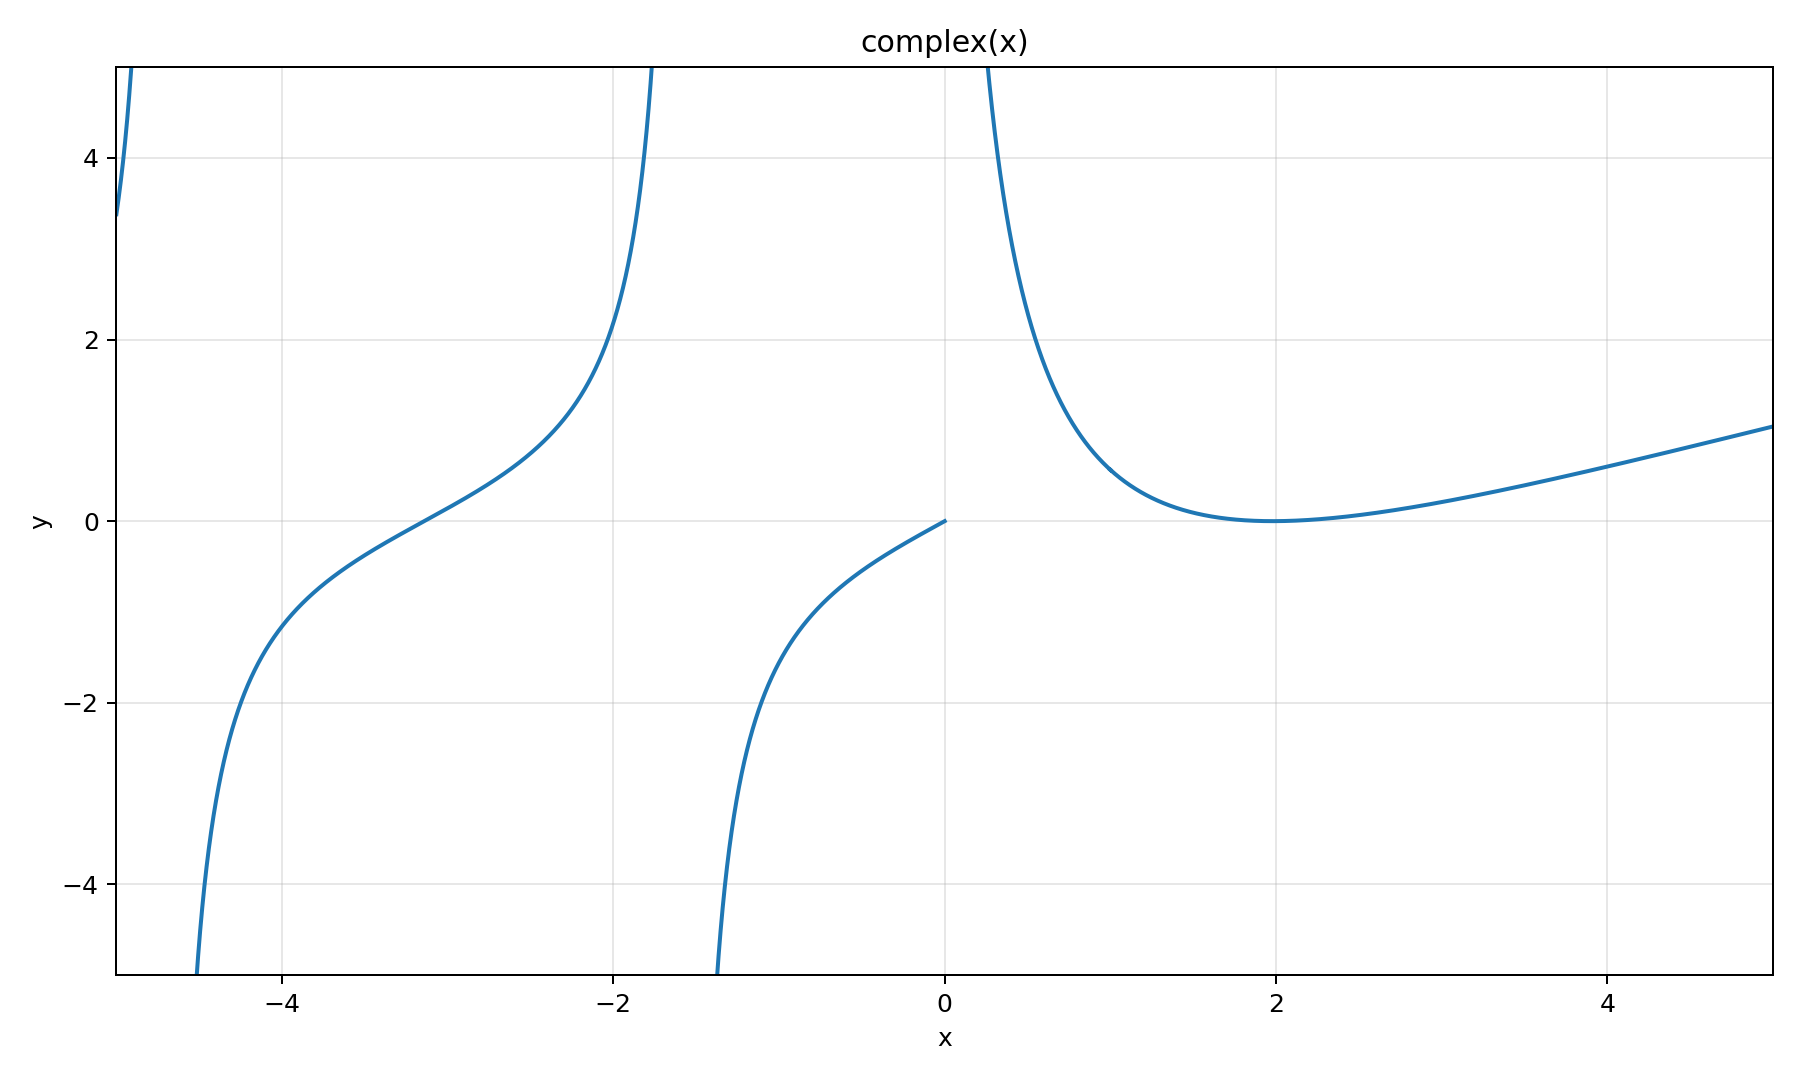
\includegraphics[width=0.75\textwidth]{assets/complex.png} \\
    \footnotesize{График системы функций}
\end{center}

\begin{center}
    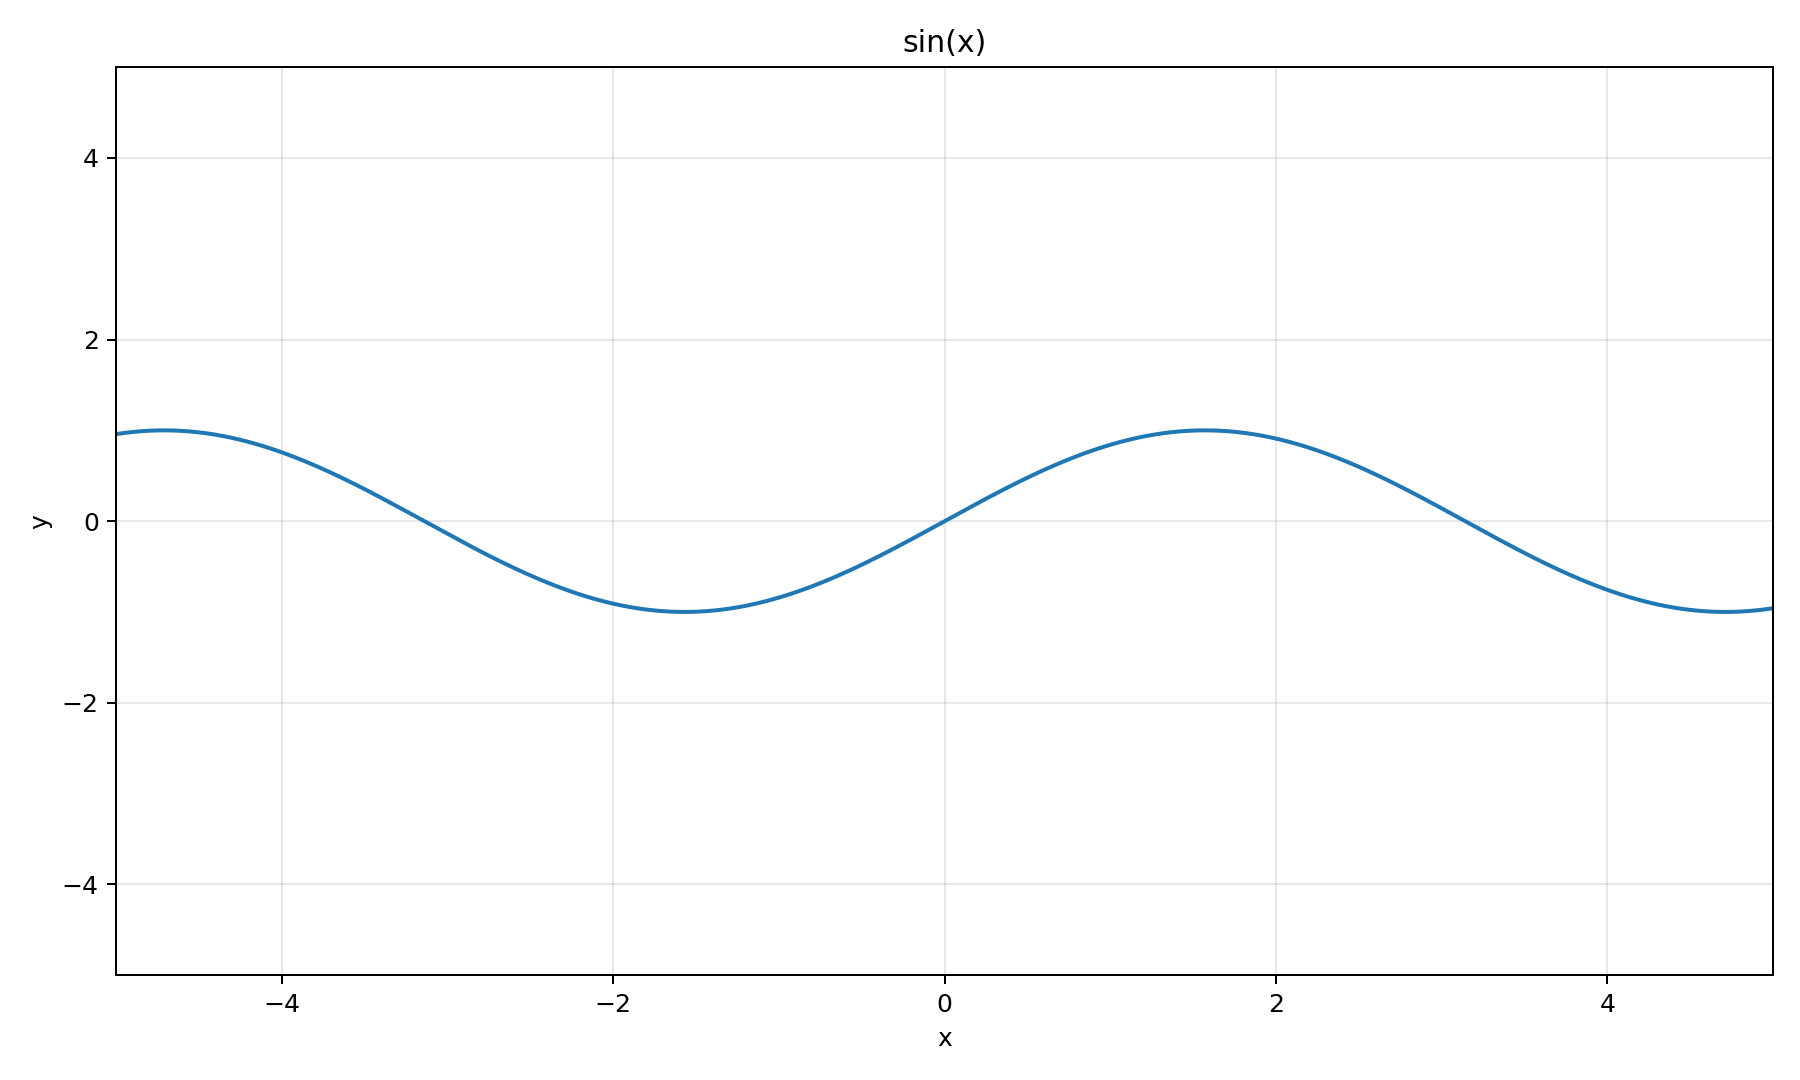
\includegraphics[width=0.75\textwidth]{assets/sin.png} \\
    \footnotesize{График $\sin x$}
\end{center}

\begin{center}
    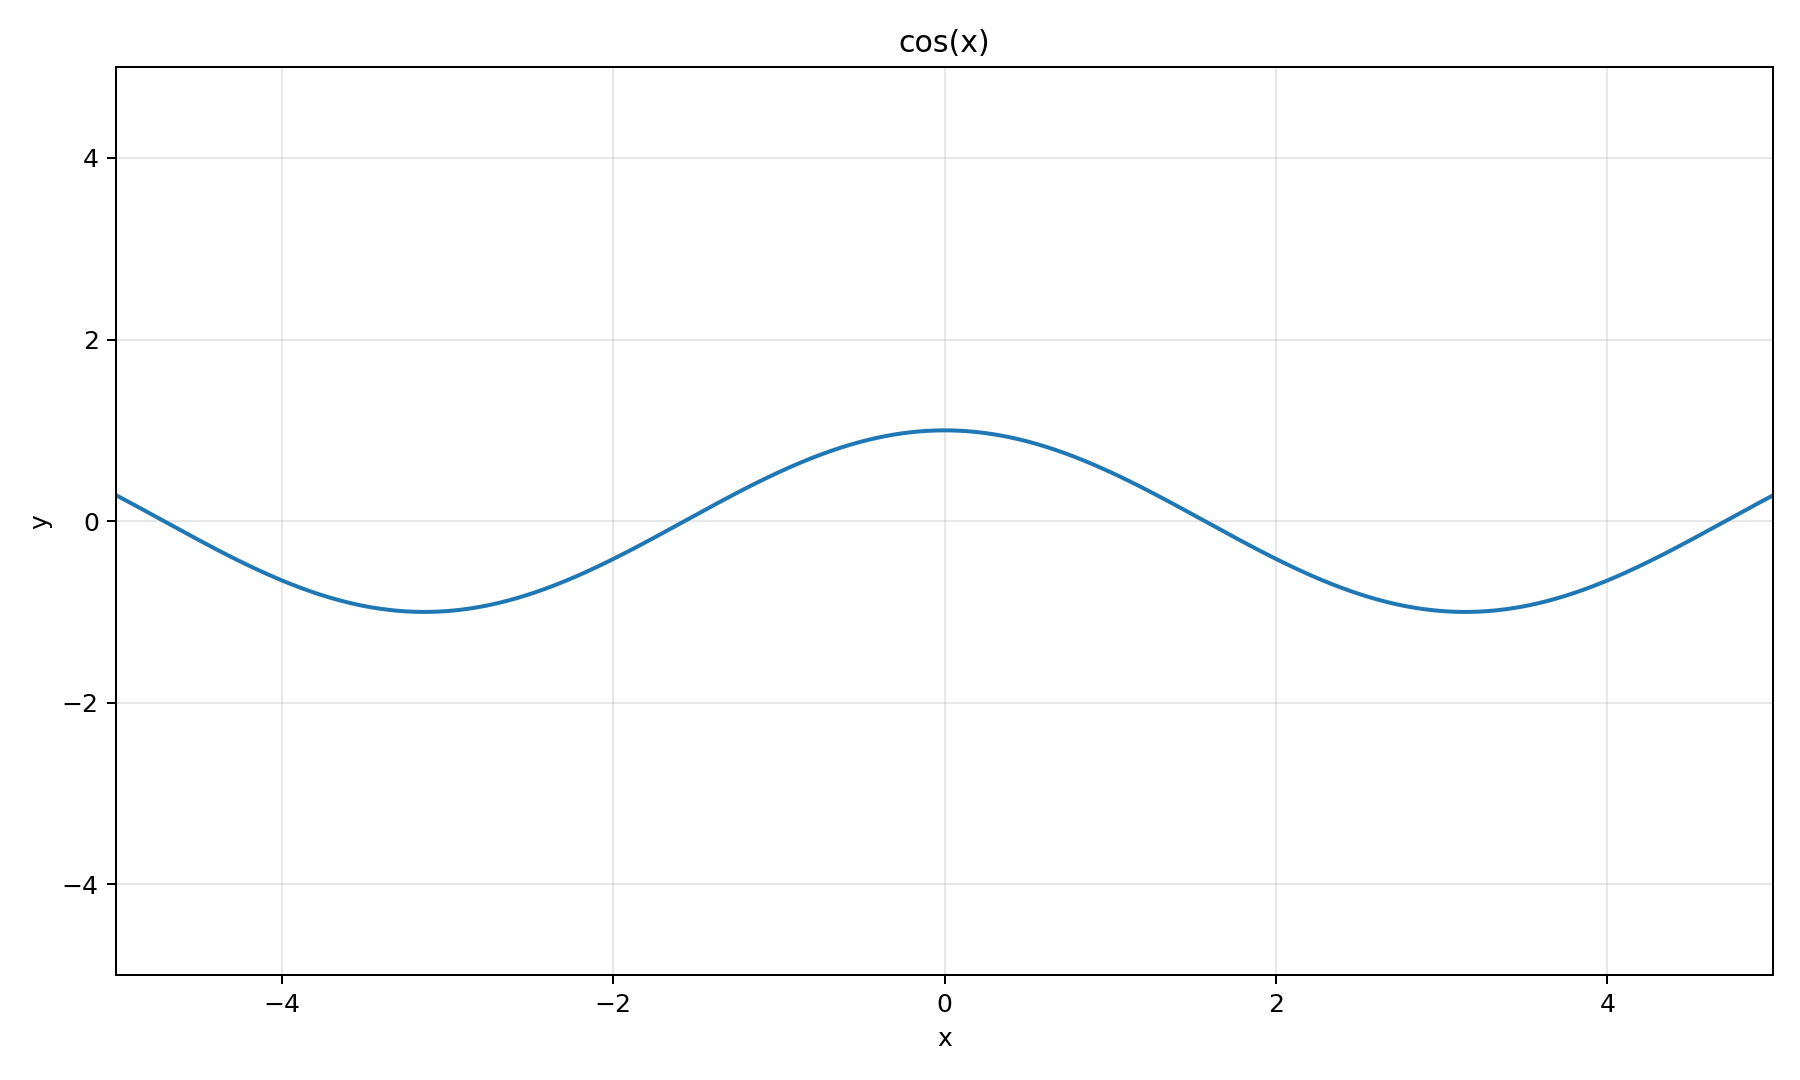
\includegraphics[width=0.75\textwidth]{assets/cos.png} \\
    \footnotesize{График $\cos x$}
\end{center}

\begin{center}
    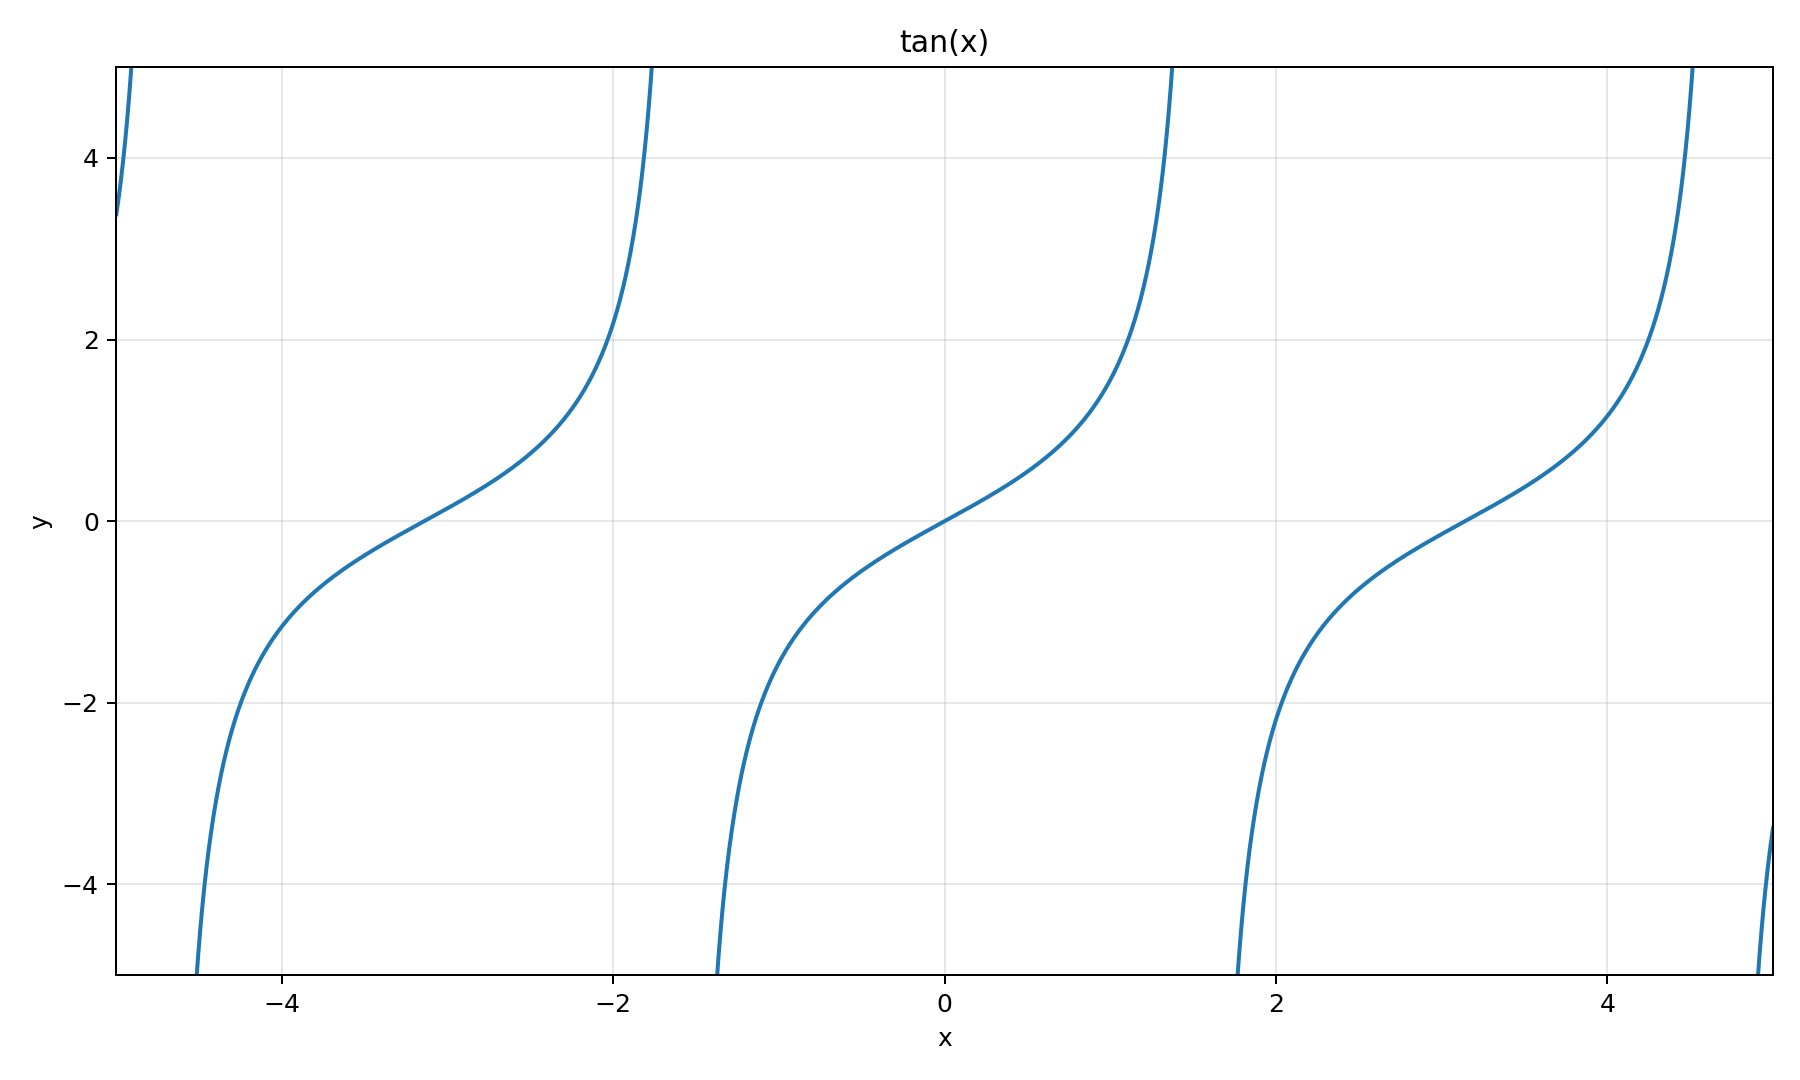
\includegraphics[width=0.75\textwidth]{assets/tan.png} \\
    \footnotesize{График $\tan x$}
\end{center}

\begin{center}
    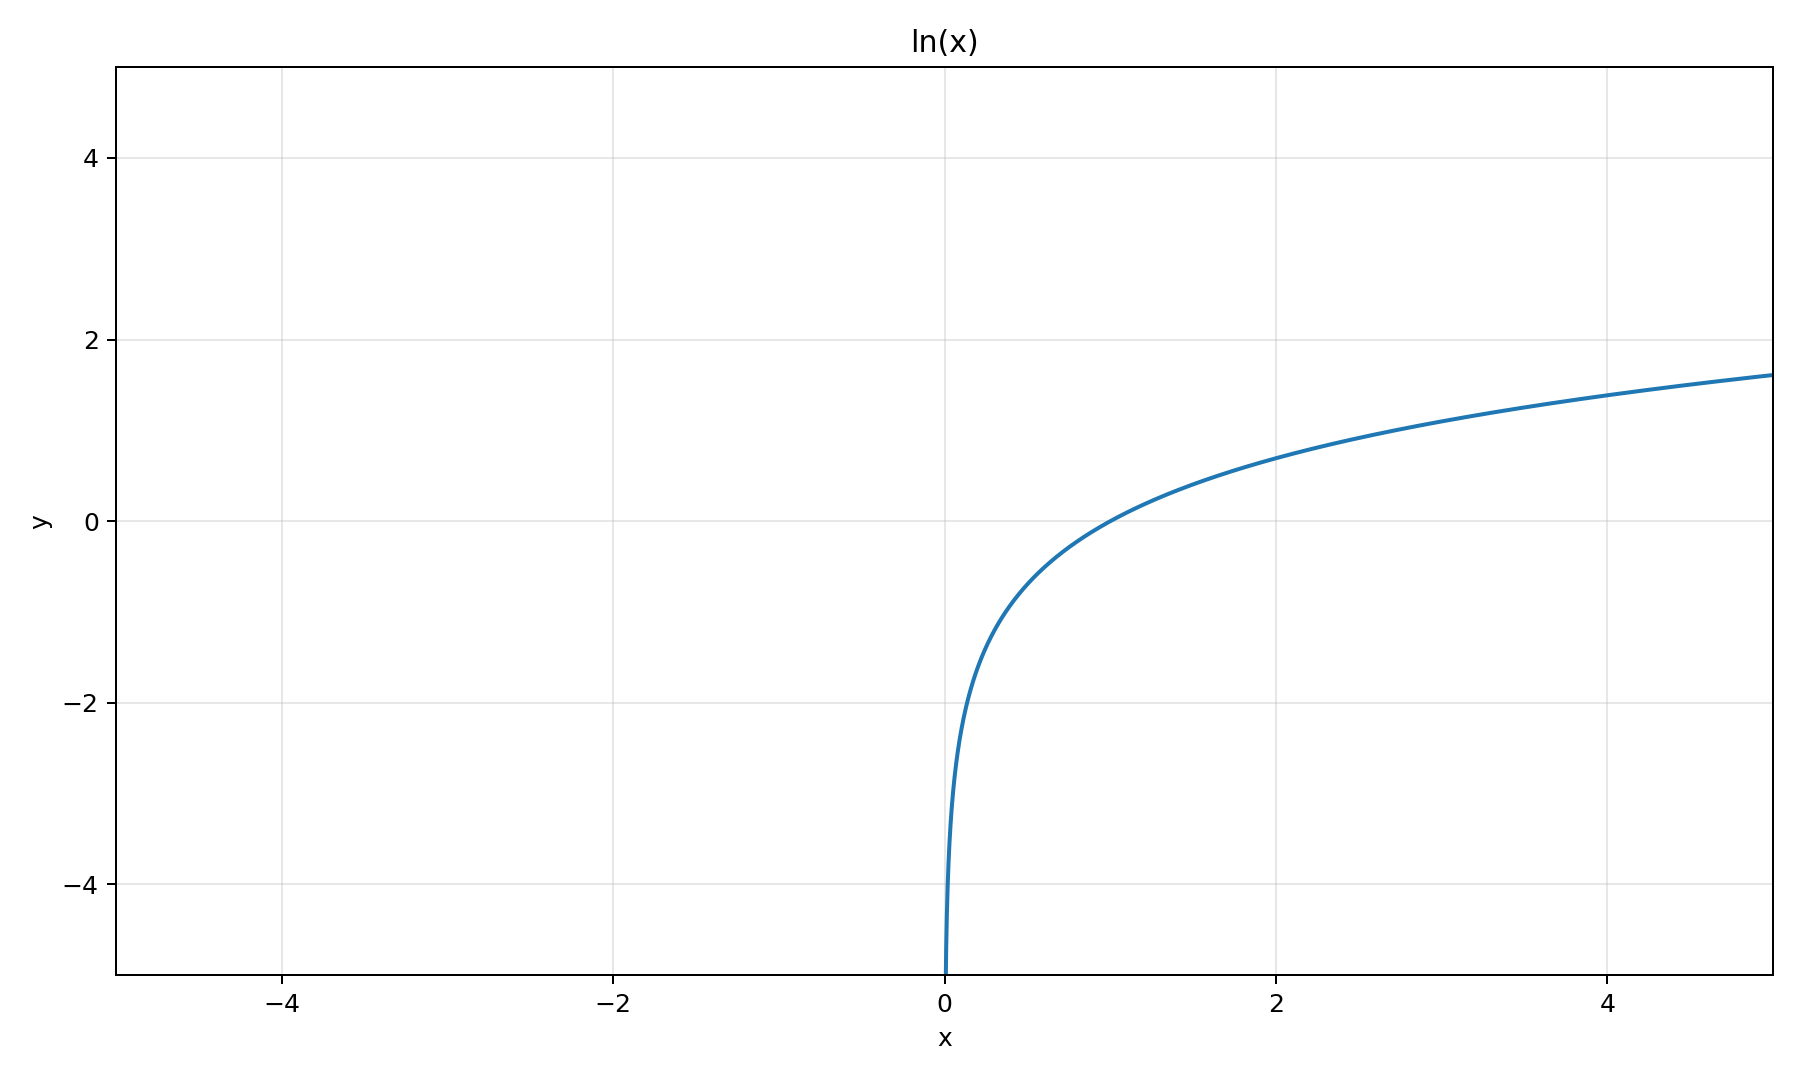
\includegraphics[width=0.75\textwidth]{assets/ln.png} \\
    \footnotesize{График $\ln x$}
\end{center}

\begin{center}
    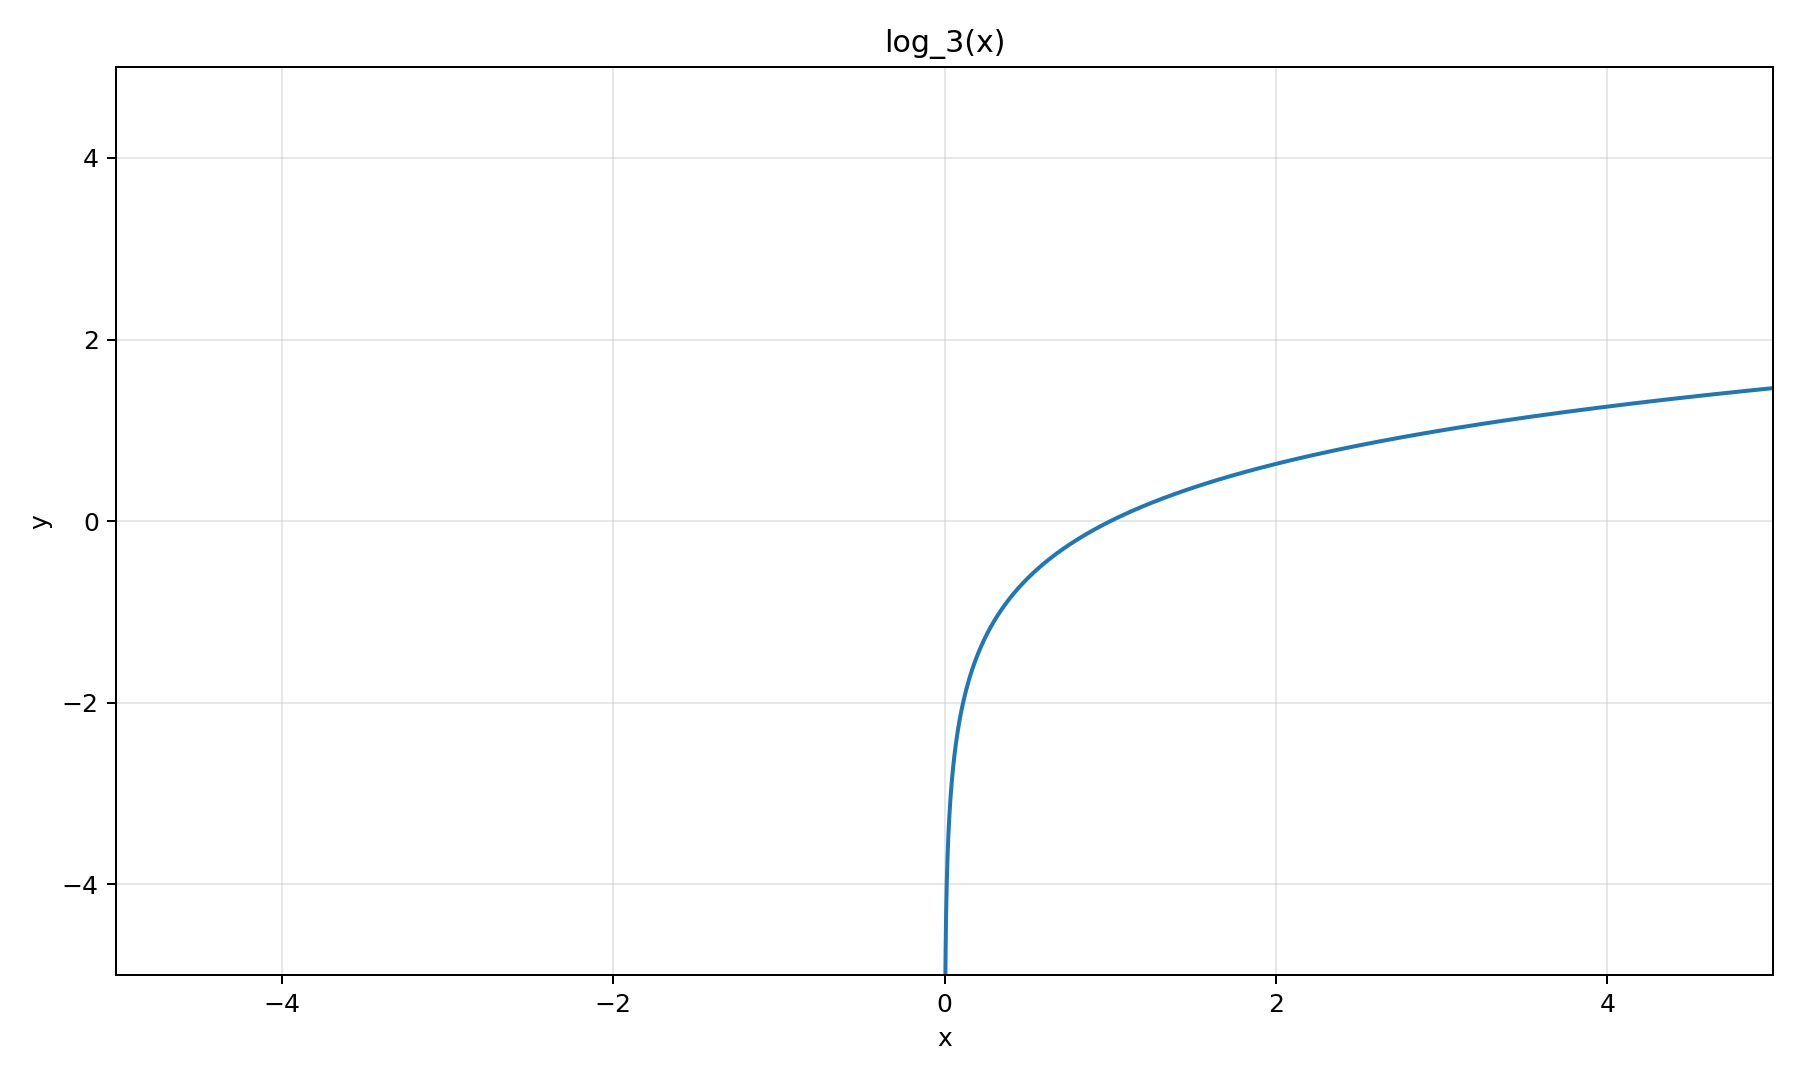
\includegraphics[width=0.75\textwidth]{assets/log_3.png} \\
    \footnotesize{График $\log_3 x$}
\end{center}

\begin{center}
    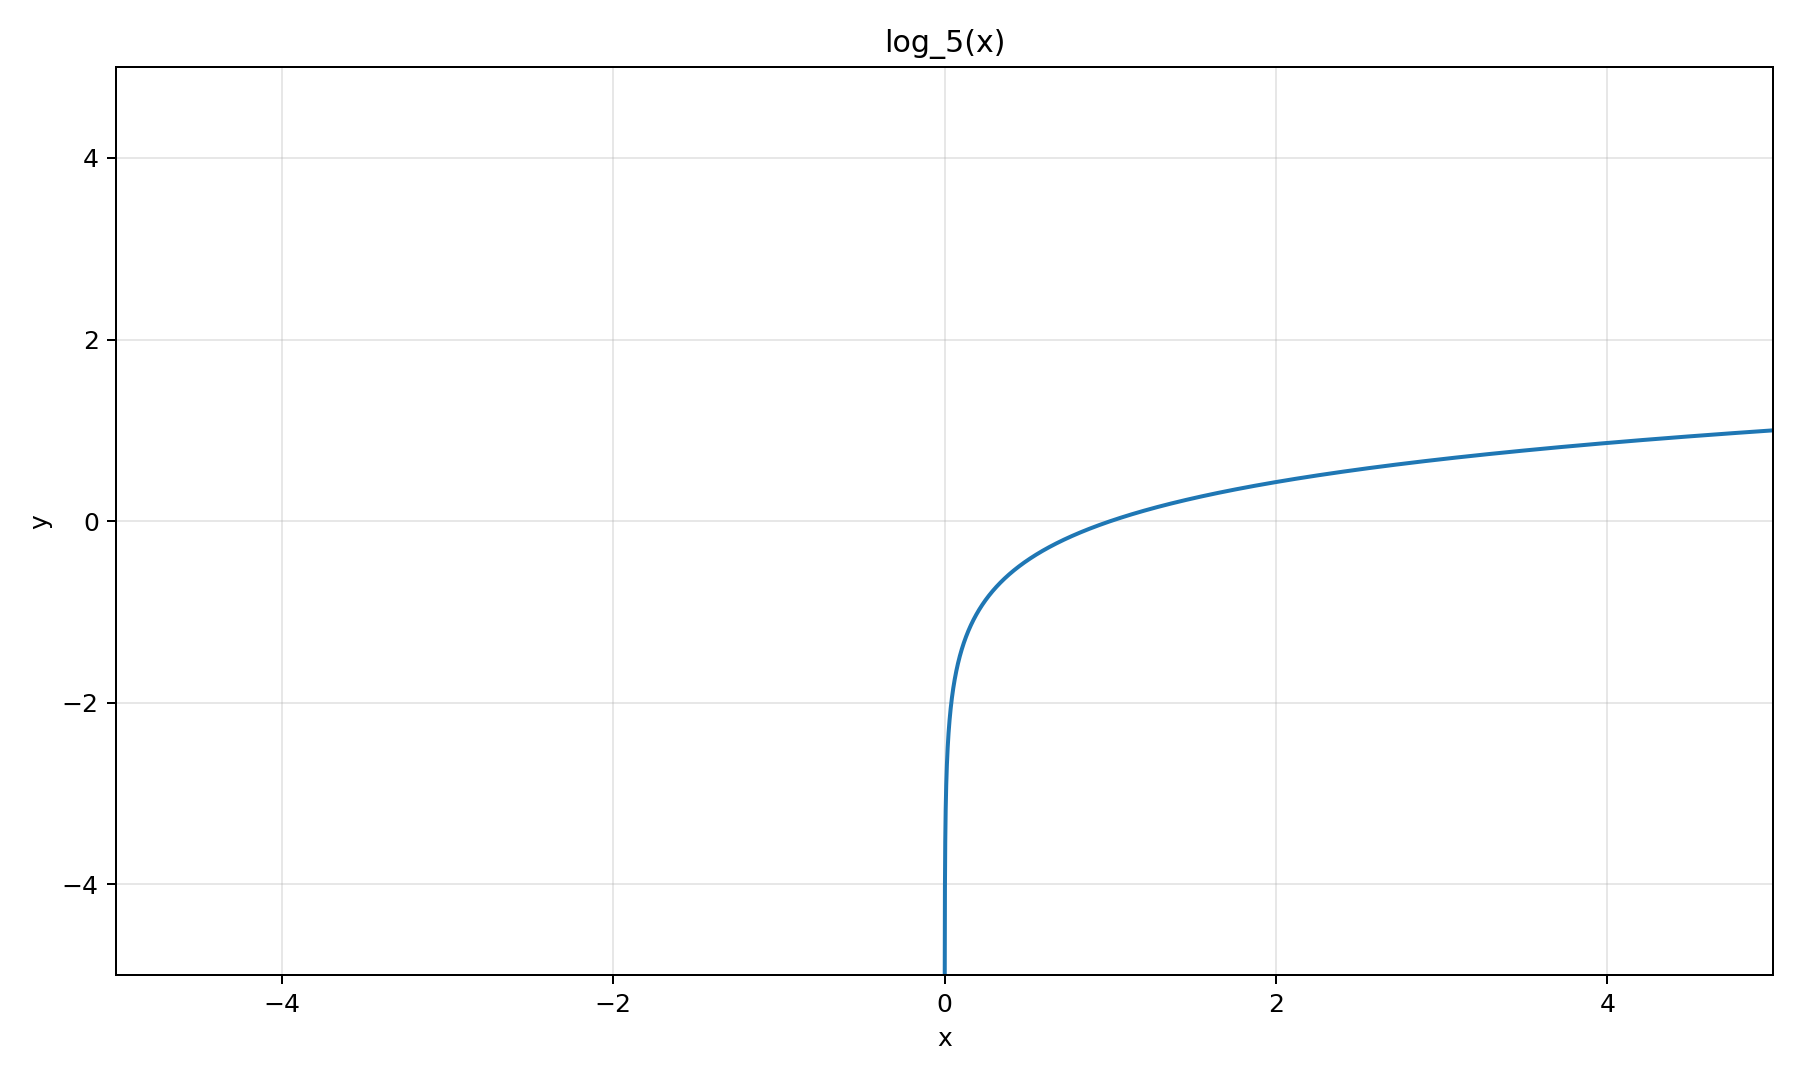
\includegraphics[width=0.75\textwidth]{assets/log_5.png} \\
    \footnotesize{График $\log_5 x$}
\end{center}
\pagebreak
\section*{Выводы}
Я познакомился с методами и стратегиями интеграционного тестирования и разработал
тестовые покрытие для системы функций
\end{document}
